\documentclass[12pt,a4paper,oneside]{report}
\usepackage[spanish]{babel}
\selectlanguage{spanish}
\usepackage[T1]{fontenc}
\usepackage{times}
\usepackage[utf8]{inputenc}
\usepackage{amsmath}
\usepackage{graphicx}
\usepackage{multicol}
\usepackage{longtable}
\usepackage[refpages]{gloss}
\usepackage{float}
\usepackage{bigstrut}
\usepackage{appendix}
\usepackage{lscape} 
\usepackage{pdflscape}
\usepackage{multirow}
\usepackage{listings}
\usepackage{color}
\usepackage{setspace}
\usepackage{enumerate} 
\usepackage{ragged2e}
\usepackage{comment}
\usepackage{fixltx2e}
\usepackage{caption}
\usepackage{subcaption}
\usepackage{parskip} % Espaciado entre párrafos
\usepackage{titlesec}
\usepackage{hyperref}
\usepackage{url}
\usepackage{textcomp}
\usepackage{wasysym}
\usepackage[margin=3cm]{geometry} % Ajuste de márgenes
\usepackage{apacite}
\usepackage{array} % necesario si usas newcolumntype

% Configuración de columnas
\newcolumntype{P}[1]{>{\centering\arraybackslash}m{#1}} % Para modificar tablas
\captionsetup[table]{skip=10pt} % Espacio debajo de las tablas
\bibliographystyle{apacite}

% Configuración de fuente y espaciado
\onehalfspacing % Espacio entre líneas
\setlength{\parskip}{12pt} % Espacio entre párrafos
\setlength{\parindent}{0pt} % Sin sangría en los párrafos

% Configuración de títulos y capítulos
\renewcommand{\BOthers}[1]{et al.\hbox{}}
\renewcommand\bibname{Bibliografía}
\renewcommand*{\contentsname}{Índice}
\renewcommand*{\listtablename}{Índice de tablas}
\renewcommand*{\listfigurename}{Índice de figuras}
\renewcommand{\appendixname}{Anexos}
\renewcommand{\appendixtocname}{Anexos}
\renewcommand{\appendixpagename}{Anexos}
\renewcommand{\thetable}{\arabic{chapter}.\arabic{table}}
\renewcommand*{\tablename}{Tabla}
\renewcommand{\chaptername}{Capítulo}
\renewcommand{\thechapter}{\arabic{chapter}}
\renewcommand{\thesection}{\arabic{chapter}.\arabic{section}}
\renewcommand{\figurename}{Figura}
\renewcommand{\thefigure}{\arabic{chapter}.\arabic{figure}}
\renewcommand{\theequation}{\arabic{chapter}.\arabic{equation}}
\spanishdecimal{.}

\begin{document}

% Numeración romana para las primeras páginas
\pagenumbering{roman}

% Carátula
\begin{titlepage}
    \begin{center}
        {\Large \bf PONTIFICIA UNIVERSIDAD CATÓLICA DEL PERÚ}\\
        \vspace{8mm} 
        {\Large FACULTAD DE CIENCIAS E INGENIERÍA}\\
        
        % Logo de la universidad
        \begin{figure}[H]
            \centering
            
\includegraphics[width=15cm]{Imagenes/logopucp.png} % Asegúrate de que la ruta y el nombre del archivo sean correctos
        \end{figure}
        
        % Título de la tesis
        {\Large \bf ANÁLISIS TIEMPO-HISTORIA NO LINEAL} \\[0.3 cm]
        {\Large \bf DE UN EDIFICIO DE 8 PISOS CON PROGRAMACIÓN} \\[0.3 cm] 
        {\Large \bf INTERACTIVA CON PYTHON Y OPENSEES}\\
        
        \vspace{1 cm}
        
        % Descripción del trabajo
        {\large Tesis para obtener el título profesional de}\\[0.5cm]
        {\large \bf INGENIERO CIVIL}\\[1.0cm]
        
        % Autor y asesor
        {\large \bf AUTOR}\\[0.5 cm] 
        {\large Daniel Octavio Xavier Medina Quispe}\\[0.7 cm] 
        {\large \bf ASESOR}\\[0.5 cm] 
        {\large Ing. José Martín Velásquez Vargas}\\

        \vspace{1.3 cm}
        
        % Fecha
        {Lima, \today}
    \end{center}
\end{titlepage}

% Dedicatoria
\begin{titlepage}
    \begin{center}
        
        {\large \bf DEDICATORIA}\\[1cm]
        \vspace*{13cm} % Ajusta el espacio superior para centrar verticalmente el contenido
        
        \begin{flushright}
            \textit{A mis padres, por el gran apoyo incondicional}\\[0.5cm]
            \textit{en todo momento y compresión en todas las etapas de mi vida}\\[1.5cm]
            \textit{A mis amigos por el apoyo emocional y motivación}\\[0.5cm]
            \textit{para poder culminar este proyecto de tesis}\\[0.5cm]
            
            \end{flushright}
        
        \vfill % Relleno vertical para ajustar el contenido en la página
    \end{center}
\end{titlepage}


% Agradecimientos
\begin{titlepage}
    \begin{center}
        
        {\large \bf AGRADECIMIENTOS}\\[1cm]
        \vspace*{13cm} % Ajusta el espacio superior para centrar el contenido verticalmente
        
        \begin{flushright}

            \textit{A mi estimado asesor Diego Villagomez , por su tiempo}\\[0.5cm]
            \textit{ y conocimiento brindado}\\[1.5cm]
            \textit{A mi jefe de grupo Andrés Perez y compañeros por tantas enseñanzas}\\[0.5cm]
            \textit{ y momentos agradables}\\[0.5cm]
            \end{flushright}

        \vfill % Relleno vertical para ajustar el contenido en la página
    \end{center}
\end{titlepage}


% Resumen
\chapter*{\centering \large RESUMEN} 
%\addcontentsline{toc}{chapter}{Resumen} % si queremos que aparezca en el índice
\markboth{Resumen}{Resumen} % encabezado
\onehalfspacing
\setlength{\parskip}{1em} % Ajusta el espacio entre párrafos

{
Para realizar el diseño de una edificación, se hace un modelo y un análisis estructural que nos permite predecir el comportamiento de la estructura ante las solicitaciones de servicio, sísmicas, entre otros. Para realizar este análisis, las técnicas ingenieriles realizan demasiadas asunciones que simplifican los cálculos. Sin embargo, no se tiene una forma de medir la veracidad de estos resultados de forma experimental. Los diseños se basan en la experiencia y criterio del ingeniero a cargo, pero este conocimiento puede fallar.

Por este motivo, las normas de construcción peruana nos indican que tenemos que aplicar un sobrediseño para tener un factor de seguridad, lo cual encarece el proyecto. Esta tesis tiene como objetivo desarrollar una herramienta, con interfaz gráfica, de fácil uso e interpretación, en Python, que permita medir la confiabilidad de los resultados del análisis estructural hallados con métodos discretos (exactos). En otras palabras, medir la probabilidad de ocurrencia de los resultados hallados previamente.

Este análisis de confiabilidad estructural se realizará con la librería de Python OpenSeesPy, la cual realizará el análisis estructural; seguidamente se agregará la variabilidad a las propiedades de la estructura y solicitaciones (señales sísmicas, propiedades de concreto, variaciones en construcción, entre otros).
}


% Índices
\tableofcontents \newpage
\listoffigures \newpage
\listoftables \newpage

\makegloss
\newpage

% Numeración arábiga para el resto del documento
\pagenumbering{arabic}

% Capítulos
\chapter{Introducción}

\section{Planteamiento del problema}
Los criterios de diseño, ya sea en concreto armado, en acero o en cualquier otro material, se basan en la normativa de construcción. En esta normativa se presentan ciertos criterios y requisitos mínimos para la construcción de diferentes obras. Estos criterios están sustentados en los resultados experimentales de diferentes ensayos, experiencia pasada y nuevos métodos de análisis computacional. 

Sin embargo, para el caso de diseño sismorresistente, los criterios son difíciles de corroborar y sustentar experimentalmente, ya que los ensayos para este tipo de solicitación no son posibles a nivel real de la estructura debido a la magnitud, los recursos o el tiempo. Por este motivo, las normas de diseño sismorresistente se basan principalmente en la experiencia de anteriores eventos sísmicos.

En el Perú, la norma técnica que rige los criterios de construcción para solicitaciones de sismo es la norma peruana E.030 de Diseño Sismorresistente. Este documento presenta métodos de calificación de estructuras, peligro sísmico por zonas y el comportamiento esperado ante un sismo, entre otras cosas. A pesar de lo indicado en la norma, existe una alta posibilidad de que la respuesta final de la estructura no esté contemplada en el documento. Esto se debe a que los sismos son eventos aleatorios y, como se mencionó anteriormente, la norma se basa en la experiencia de eventos sísmicos pasados. Sin embargo, en el Perú no existen registros de suficientes eventos sísmicos para alcanzar un nivel adecuado de confiabilidad.

Además de este problema, en la norma E.060 de Concreto Armado, el material más usado para la construcción en el mundo, se mencionan propiedades del concreto, como la resistencia a la compresión (\textit{f'c}) y el módulo de Young. Estas propiedades no tienen un valor constante, sino que varían de acuerdo con la calidad de las materias primas. Además de esto, se debe considerar la variabilidad de los métodos de construcción utilizados en la ejecución de la obra. 

Toda esta variabilidad en las propiedades, características, dimensiones, métodos de construcción, modelos de análisis, limitaciones computacionales y la aleatoriedad de los eventos sísmicos produce una desconfianza en los resultados utilizados para el diseño de estructuras. Como contramedida a esta situación, las normas indican la sobrerresistencia de los elementos estructurales. Sin embargo, esta solución, aunque viable y comprobada, encarece el proyecto final tanto a nivel económico como de tiempo. Cabe agregar que esta sobrerresistencia, también considerada como el factor de seguridad, brinda un falso nivel de confianza, ya que, como se mencionó anteriormente, los eventos aleatorios y las propiedades variables hacen que la respuesta de la estructura frente a estas cargas sea incierta, incluso llegando a casos extraordinarios donde la estructura podría colapsar.

La presente propuesta surge a partir de la problemática mencionada y presenta una metodología y herramientas digitales para realizar una medición de la confiabilidad estructural.

\section{Antecedentes y justificación}
La ingeniería sismorresistente es una de las ramas más recientes de la ingeniería civil. Uno de sus objetivos es que las obras civiles no colapsen ante eventos sísmicos y que puedan asegurar el resguardo de la vida (Muñoz, 2020). A lo largo de la historia del Perú, se han creado normas de diseño que buscan cumplir este objetivo, proporcionando parámetros mínimos para garantizar un comportamiento adecuado. 

Una de las primeras recomendaciones para el diseño sismorresistente se oficializó en 1977 en la normativa peruana de construcción. En 1996, se produjo el sismo de Nasca, de magnitud 7.7 Mw, que causó la destrucción de colegios y viviendas en toda la zona. A raíz de este evento, se creó la norma sismorresistente de 1997. Sin embargo, en 2001 ocurrió un sismo en la localidad de Arequipa, con una magnitud de 7.9 Ms, que dejó muchos colegios inutilizables, lo cual evidenció que la norma no contemplaba muchos aspectos de las unidades escolares. Este evento marcó el inicio de la redacción de una nueva norma sismorresistente, publicada en 2003. A lo largo de los años, se publicó una versión de la norma en 2016 y, la actualmente vigente, en 2018.

En cada una de las normas antes mencionadas, los eventos sísmicos han proporcionado información valiosa para mejorar, corregir y reescribir la normativa de diseño sismorresistente. Sin embargo, este enfoque limita mucho la implementación de nuevas metodologías de construcción y diseño. Por este motivo, en este documento se plantea una metodología para realizar simulaciones sísmicas y comparaciones de modelos estructurales. Adicionalmente, se incluye una medición de confiabilidad estructural.

Contar con resultados de confiabilidad permite reducir los factores de seguridad, ya que, al realizar un análisis de confiabilidad, se tiene una mejor seguridad del comportamiento real. Al reducir los factores de seguridad, el proyecto de construcción disminuirá sus costos económicos y aumentará la seguridad de la edificación.

\section{Hipótesis}
Se asume que la deriva de un edificio al aplicar una carga lateral aleatoria está directamente relacionada con dicha carga; por lo tanto, el análisis probabilístico nos dará resultados similares a los de un análisis discreto.

\section{Objetivos}
El objetivo general de la tesis es brindar una herramienta para realizar un análisis de confiabilidad estructural.

Los objetivos específicos del proyecto son:
\begin{itemize}
    \item Verificar la fiabilidad de los resultados hallados por métodos discretos mediante la probabilidad de ocurrencia de estos.
    \item Aplicar técnicas de programación orientada a objetos y simulación aleatoria.
    \item Crear un programa para obtener señales sísmicas sintéticas.
    \item Aplicar técnicas de muestreo para la optimización del análisis de confiabilidad.
\end{itemize}

\chapter{Marco teórico y metodología}

\section{Marco teórico}
La vulnerabilidad de una estructura se puede definir como la probabilidad de ocurrencia (predisposición) de sufrir daños ante la ocurrencia de un movimiento sísmico \cite{bonett2003}. El peligro sísmico se puede definir como la probabilidad de ocurrencia de movimientos sísmicos durante una cierta cantidad de vida útil \cite{bommer1998}. Añadido a esto, se puede definir el riesgo sísmico como:
\begin{equation}
\text{Riesgo} = \text{Peligro} \times \text{Vulnerabilidad}.
\end{equation}

Para realizar un análisis de confiabilidad de estructuras, se propone un análisis estocástico no determinístico. El análisis estocástico hace un análisis de variables aleatorias dependientes de una variable en común, como el tiempo, que afectan al sistema evaluado \cite{ramirez2007}. Este tipo de análisis se ha utilizado anteriormente para la generación de señales sintéticas y aún no se ha implementado en otros procesos de análisis debido al costo computacional que implica.

Además de ello, se requiere un análisis no lineal de las estructuras; es decir, donde la fuerza y el desplazamiento no se relacionan linealmente \cite{hanganu1997}. Este análisis no lineal requiere un motor de análisis muy potente como es el OpenSees. En este caso, se hará uso del lenguaje de programación Python y del entorno de desarrollo integrado (IDE) Visual Studio Code. Adicionalmente, se utilizará la librería OpenSeesPy \cite{zhu2018}, una versión de OpenSees para Python. Dentro del intérprete mencionado se compilará un código para el modelo y el análisis de una estructura sometida a una carga sísmica. 

Sin embargo, para la medición de la confiabilidad estructural, se debe agregar la variabilidad de las propiedades y las cargas. Para realizar este muestreo, se hará uso de la simulación de Monte Carlo. Cabe recalcar que, para realizar una mejor simulación aleatoria, se debe llevar a cabo un muestreo adecuado y una cantidad suficiente de simulaciones.

Todas estas tareas mencionadas requieren una alta potencia computacional debido a la cantidad de datos a analizar. Por este motivo, se hace uso de técnicas de muestreo para obtener la mejor representatividad de la muestra a estudiar con la menor cantidad de ejemplares. Finalmente, se realiza un proceso de selección y filtración para obtener los resultados finales de la confiabilidad. Todo este proceso será integrado en un programa con interfaz gráfica desarrollada en Python con la librería PySide6. Esto nos permitirá tener una mejor visualización y comprensión de los resultados.

\section{Conceptos relacionados}
\subsection{Fenómeno sísmico}
Los eventos sísmicos en el Perú son producidos por la subducción de la placa de Nazca bajo la placa Sudamericana. Este proceso provoca perturbaciones súbitas en el interior de la Tierra, que se transmiten hacia la corteza terrestre, donde se originan los eventos sísmicos. En otras palabras, un sismo ocurre cuando existe movimiento relativo entre las placas en cuestión. Como estas están en contacto, generan fricción y liberan energía. Este evento es de tipo aleatorio; es decir, no se sabe cuándo podría ocurrir un evento sísmico. Esto se debe a que estos eventos se originan a gran profundidad, lo cual imposibilita su observación y posible predicción.

A lo largo de la historia, se han propuesto muchos métodos, técnicas y análisis probabilísticos para la predicción de los sismos. Sin embargo, cada uno de estos ha fallado y, hasta ahora, solo se puede realizar una estimación de la magnitud del sismo venidero utilizando el registro histórico de sismos. Datos como la localización o la fecha estimada de ocurrencia son muy difíciles de predecir. La razón es que no se pueden localizar con precisión las zonas de acumulación de energía. Se han creado mapas para estimar estas zonas; sin embargo, no son muy precisos y siempre tienen un margen de incertidumbre. Además, la liberación de energía es muy rápida, lo que hace muy difícil advertir o colocar una alarma con un tiempo respetable para resguardar a las personas.

\subsection{Confiabilidad estructural}
La confiabilidad estructural es la probabilidad de que un sistema funcione adecuadamente durante su periodo de vida \cite{choi2006}. Extrapolando este concepto a la ingeniería civil, se puede decir que la confiabilidad estructural es la probabilidad de no sobrepasar el estado límite, teniendo factores de seguridad que aseguren la función de las obras civiles. Para realizar este análisis se utilizan técnicas de probabilidad que afectan la respuesta de la estructura ante solicitaciones externas. Este es un nuevo enfoque para proporcionar herramientas de diseño. El siguiente cuadro muestra una comparación entre los dos enfoques de diseño.

\begin{figure}[H]
    \centering
    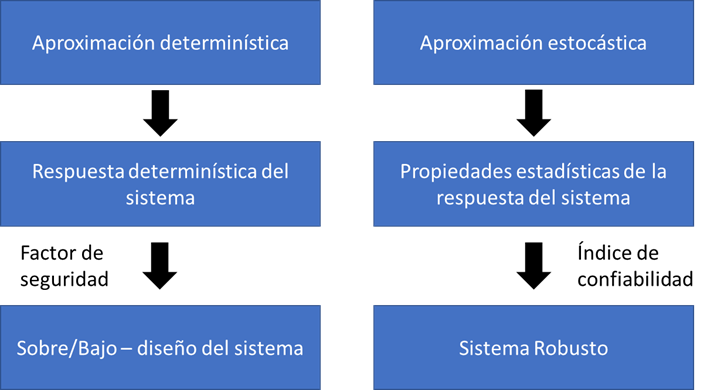
\includegraphics[width=0.8\textwidth]{Imagenes/figure1.png} % Reemplazar con la ruta correcta de la imagen
    \caption{Herramientas para el diseño bajo un análisis de incertidumbre. Tomado de \protect\cite{choi2006}}
    \label{fig:design_tools}
\end{figure}

\subsubsection{Simulación Monte Carlo}
La simulación de Monte Carlo es un método de muestreo o método estadístico de prueba. Esta simulación consiste en la evaluación de un sistema generando variables aleatorias \cite{choi2006}. Es una herramienta muy utilizada que permite medir la probabilidad de ocurrencia de ciertos eventos en un sistema. 

Sin embargo, esta simulación requiere una gran cantidad de muestras para que los resultados finales sean convergentes. Experimentalmente, se ha observado que el número mínimo es de 2000 simulaciones para obtener un resultado aproximado. Esto hace que sea un método muy costoso a nivel computacional para sistemas muy complejos, donde se pueden tener \(n\) variables aleatorias. Por este motivo, se han desarrollado varios métodos de obtención de muestras que permiten tener una mejor representatividad y realizar la simulación de Monte Carlo con menos ejemplares.

\subsubsection{Hiper Cubo Latino}
El Hiper Cubo Latino es un método de muestreo estratificado que consiste en cuatro pasos:
\begin{itemize}
    \item Dividir la distribución de probabilidad de la variable aleatoria en \(n\) partes con la misma probabilidad de ocurrencia.
    \item Seleccionar un valor representativo de cada uno de los \(n\) tramos generados previamente. El criterio de selección puede variar según cada caso.
    \item Repetir los dos pasos anteriores para las diferentes variables que se tengan.
    \item Finalmente, relacionar cada punto elegido en los \(n\) tramos de cada variable.
\end{itemize}

Este método de muestreo permite reducir significativamente el número de simulaciones a realizar en un sistema. En la Figura \ref{fig:latin_hypercube}, se muestra cómo se relacionan dos variables usando este método. Para la creación de la distribución de probabilidades de cada variable, se tuvo que simular aproximadamente 10,000 muestras. Sin el método del Hiper Cubo Latino, se tendría que analizar el sistema cerca de 10,000 veces para obtener resultados representativos. Sin embargo, con este método, simplemente se realiza el análisis del sistema 14 veces, ya que la muestra utilizada es más representativa.

\begin{figure}[H]
    \centering
    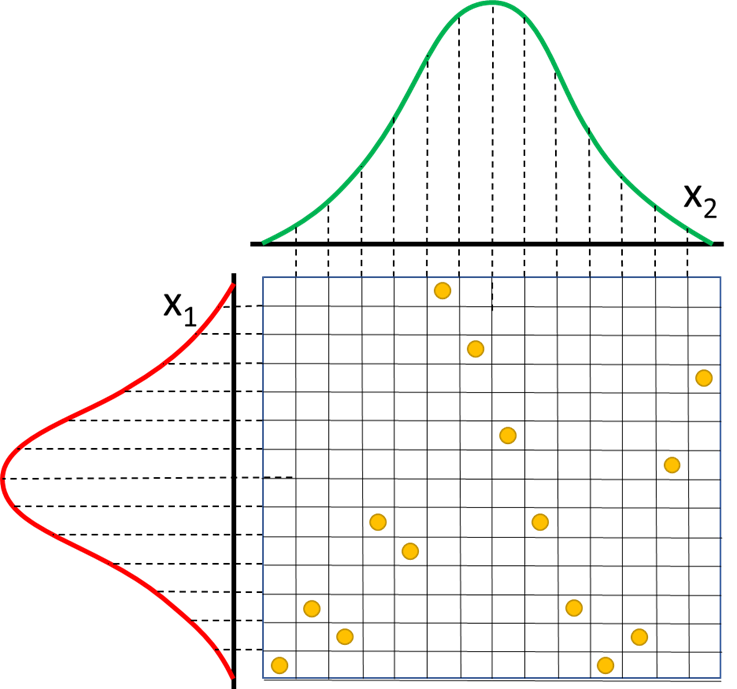
\includegraphics[width=0.8\textwidth]{Imagenes/figure2.png} % Reemplazar con la ruta correcta de la imagen
    \caption{Concepto básico del Hiper Cubo Latino: Dos variables con 14 divisiones.}
    \label{fig:latin_hypercube}
\end{figure}

\subsubsection{Métodos de confiabilidad}
\textbf{Método de segundo momento de primer orden (FOSM)}\\
En este método se realiza el cálculo de confiabilidad (\(\beta\)) dividiendo el valor promedio de la función de falla entre la desviación estándar de estas. La función de falla está definida por la siguiente expresión:

\begin{equation}
\tilde{g}(X) \approx g(\mu_X) + \nabla g(\mu_X)^T (X_i - \mu_{X_i}),
\end{equation}

donde \(\mu_X = \{\mu_{X_1}, \mu_{X_2}, \mu_{X_3}, \dots, \mu_{X_n}\}^T\) y \(\nabla g(\mu_X)\) es el gradiente de \(g\) evaluado en \(\mu_X\):

\begin{equation}
\nabla g(\mu_X) = \left\{ \frac{\partial g(\mu_X)}{\partial X_1}, \frac{\partial g(\mu_X)}{\partial X_2}, \dots, \frac{\partial g(\mu_X)}{\partial X_n} \right\}^T.
\end{equation}

El valor promedio de la aproximación de la función del estado límite \(\tilde{g}(X)\) es:

\begin{equation}
\mu_{\tilde{g}} \approx E[g(\mu_X)] = g(\mu_X).
\end{equation}

La variación aproximada del estado límite de la función \(\tilde{g}(X)\) es:

\begin{equation}
\text{Var}[\tilde{g}(X)] \approx \text{Var}[g(\mu_X)] + \text{Var}[\nabla g(\mu_X)^T (X - \mu_X)].
\end{equation}

Por lo tanto, la desviación estándar de la aproximación a la función del estado límite es:

\begin{equation}
\sigma_{\tilde{g}} = \sqrt{\text{Var}[\tilde{g}(X)]} = \sqrt{[\nabla g(\mu_X)^T]^2 \text{Var}(X)} = \left[\sum_{i=1}^{n} \left(\frac{\partial g(\mu_X)}{\partial X_i}\right)^2 \sigma_{X_i}^2 \right]^{1/2}.
\end{equation}

El índice de confiabilidad se define como:

\begin{equation}
\beta = \frac{\mu_{\tilde{g}}}{\sigma_{\tilde{g}}}.
\end{equation}

Este valor de confiabilidad solo se puede definir para funciones de estado límite lineales; de no ser lineales, se debe obtener una linealización de la función original de falla en el punto de valor medio. Por lo tanto, este método también se conoce como el método de valor medio. El valor de \(\beta\) dado en la ecuación (2.6) se denomina MVFOSM (Mean Value FOSM) índice de confiabilidad.

Debido a que el método mencionado tiene limitaciones en cuanto a la precisión de los resultados y su veracidad, se han propuesto variantes que mitigan estos problemas.

\textbf{Método de Hasofer y Lind (HL) índice de seguridad}\\
Buscando el punto más probable de falla (MPP por sus siglas en inglés) en la superficie de falla del estado límite, el método planteado por Hasofer y Lind corrige las deficiencias mencionadas. Este método consiste en la normalización de la superficie.

Considerando el caso básico donde se tienen variables independientes aleatorias de resistencia \(R\) y solicitación \(S\), las cuales tienen distribuciones normales. Hasofer y Lind introducen una variable aleatoria normalizada:

\begin{equation}
\hat{R} = \frac{R - \mu_R}{\sigma_R}, \quad \hat{S} = \frac{S - \mu_S}{\sigma_S},
\end{equation}

donde \(\mu_R, \sigma_R\) y \(\mu_S, \sigma_S\) son los valores medios y las desviaciones estándar de las variables aleatorias \(R\) (resistencia) y \(S\) (solicitación), respectivamente. El estado de falla se define como \(g(R, S) = R - S = 0\). Si se grafica en el plano de las abscisas la variable \(R\) y en las ordenadas la variable \(S\), la función \(g(R, S) = R - S = 0\) se grafica como una zona límite donde se produce el estado de falla. El proceso de normalización convierte esta gráfica de falla a un plano de sistema de coordenadas (\(\hat{R}, \hat{S}\)):

\begin{equation}
g(\hat{R}, \hat{S}) = \hat{R} \sigma_R - \hat{S} \sigma_S + (\mu_R - \mu_S) = 0.
\end{equation}

Si se tienen variables de cualquier distribución ortogonal y una distribución estándar normalizada \(U = \{u_1, u_2, u_3, \dots, u_n\}^T\), resulta en un nuevo conjunto de variables normalizadas y no correlacionadas. Por lo tanto, si la superficie de falla se define como \(g(X) = 0\) en el espacio original (espacio-\(X\)), la superficie de falla para el nuevo espacio normalizado (espacio-\(U\)) está dada por la función \(g(U) = 0\). La distancia a la superficie de falla puede medirse con el índice de confiabilidad, el cual es:

\begin{equation}
\beta(U) = \left(U^T U\right)^{1/2} = \|U\|_2, \quad U \in g(U) = 0.
\end{equation}

\begin{figure}[H]
    \centering
    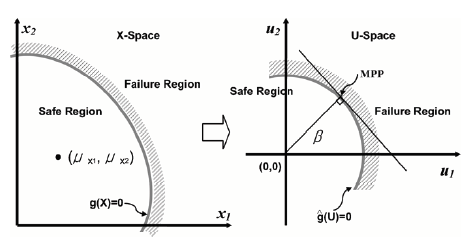
\includegraphics[width=0.8\textwidth]{Imagenes/figure3.png} % Reemplazar con la ruta correcta de la imagen
    \caption{Transformación de plano \(X\) a plano \(U\); proceso de normalización. Tomado de \protect\cite{choi2006}}
    \label{fig:normalization}
\end{figure}

El índice de confiabilidad \(\beta\) se define como la menor distancia desde el origen hasta la superficie de falla:

\begin{equation}
\beta = \min_{U \in g(U) = 0} \left(U^T U\right)^{1/2}.
\end{equation}

La ecuación (2.10) se puede resolver de muchas maneras, pero el método más empleado es el método iterativo de Hasofer y Lind, al cual Rackwitz y Fiessler modificaron para resolver variables con cualquier distribución.

El método iterativo inicia definiendo la función de falla:

\begin{equation}
g(X) = g\left(\{x_1, x_2, \dots, x_n\}^T\right) = 0.
\end{equation}

Se transforma la función de estado límite según el procedimiento previo de la ecuación (2.7):

\begin{equation}
g(U) = g\left(\{\sigma_{x_1} u_1 + \mu_{x_1}, \sigma_{x_2} u_2 + \mu_{x_2}, \dots, \sigma_{x_n} u_n + \mu_{x_n}\}^T\right) = 0.
\end{equation}

Para hallar la distancia del origen al punto de falla más probable (MPP) se hace uso de la ecuación (2.10). Para realizar este procedimiento se pueden usar series de Taylor de primer orden:

\begin{equation}
\tilde{g}(X) \approx g(U^*) + \sum_{i=1}^{n} \frac{\partial g(U^*)}{\partial U_i} (u_i - u_i^*).
\end{equation}

Se define el valor \(k\), que es el número de iteraciones del algoritmo recursivo. También se define la ecuación (2.7) para casos generales:

\begin{equation}
\frac{\partial \hat{g}(U)}{\partial u_i} = \frac{\partial g(X)}{\partial x_i} \sigma_{x_i}.
\end{equation}

Usando la ecuación (2.13), podemos obtener un valor de distancia más corta al punto de falla:

\begin{equation}
\beta = \frac{g(U^*) - \sum_{i=1}^{n} \frac{\partial g(U^*)}{\partial x_i} \sigma_{x_i} u_i^*}{\sqrt{\sum_{i=1}^{n} \left(\frac{\partial g(U^*)}{\partial x_i} \sigma_{x_i}\right)^2}}.
\end{equation}

La dirección del vector normal está dada por:

\begin{equation}
\cos \theta_{x_i} = \cos \theta_{u_i} = -\frac{\frac{\partial g(U^*)}{\partial u_i}}{|\nabla g(U^*)|} = \frac{\frac{\partial g(U^*)}{\partial u_i}}{\sqrt{\sum_{i=1}^{n} \left(\frac{\partial g(X^*)}{\partial x_i} \sigma_{x_i}\right)^2}} = \alpha_i.
\end{equation}

El valor de \(\alpha_i\) es también conocido como el \textit{factor de sensibilidad}. Expresa el efecto relativo correspondiente a una variable aleatoria en la variación total.

Finalmente, se definen los nuevos puntos para la siguiente iteración:

\begin{equation}
x_i^* = \mu_{x_i} + \beta \sigma_{x_i} \cos \theta_{x_i}, \quad (i = 1, 2, \dots, n),
\end{equation}

\begin{equation}
u_i^* = \frac{x_i^* - \mu_{x_i}}{\sigma_{x_i}} = \beta \cos \theta_{x_i}.
\end{equation}

Y se define la nueva función de falla como:

\begin{equation}
g(X) = g\left(\{x_1^*, x_2^*, \dots, x_n^*\}^T\right) = 0.
\end{equation}

En resumen, el método iterativo de Hasofer y Lind (HL) se describe de la siguiente forma:

\begin{enumerate}
    \item Definición apropiada de la función de estado límite, ecuación (2.11).
    \item Hallar el valor medio y el punto inicial de diseño, es decir, \(x_{i,k} = \mu_{x_i}\), \(i = 1, 2, \dots, n\). También se debe calcular el gradiente \(\nabla g(X_k)\). El valor de \(x_{i,k}\) se define como el \(i\)-ésimo elemento del vector \(X_k\) en la \(k\)-ésima iteración.
    \item Calcular el \(\beta\) inicial utilizando el método MVFOSM, ecuación (2.6).
    \item Hallar el nuevo punto de diseño \(X_k\) y \(U_k\) utilizando las ecuaciones (2.17) y (2.18).
    \item Calcular el nuevo valor de \(\beta\) usando la ecuación (2.15).
    \item Repetir los pasos 4 a 6 hasta que el valor de \(\beta\) alcance la convergencia.
\end{enumerate}

Para determinar el \(\beta_{HL}\) (índice de seguridad de HL) se define como:

\begin{equation}
\beta_{HL} = \min \{\beta_1, \beta_2, \dots, \beta_m\}.
\end{equation}

% ...

% Bibliografía
\bibliography{Bibliografia/library}

% Anexos
\appendix
\include{Anexos/AnexoA}
\include{Anexos/AnexoB}

\end{document}
